\hypertarget{group__porting__type}{}\section{Basic type definition}
\label{group__porting__type}\index{Basic type definition@{Basic type definition}}


file \hyperlink{vl53l0x__types_8h}{vl53l0x\+\_\+types.\+h} files hold basic type definition that may requires porting  


Collaboration diagram for Basic type definition\+:\nopagebreak
\begin{figure}[H]
\begin{center}
\leavevmode
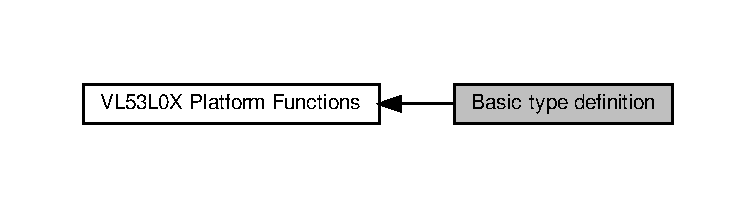
\includegraphics[width=350pt]{group__porting__type}
\end{center}
\end{figure}
file \hyperlink{vl53l0x__types_8h}{vl53l0x\+\_\+types.\+h} files hold basic type definition that may requires porting 

contains type that must be defined for the platform~\newline
when target platform and compiler provide stdint.\+h and stddef.\+h it is enough to include it.~\newline
If stdint.\+h is not available review and adapt all signed and unsigned 8/16/32 bits basic types. ~\newline
If stddef.\+h is not available review and adapt N\+U\+LL definition . 